\section{URDAD}
\label{sec:urdad}

URDAD, the {\em Use-Case, Responsibility Driven Analysis and Design} process provides an
algorithmic analysis and design process with the following characteristics:
\begin{enumerate}
  \item Both, requirements and design are step-wise refined.
  \item URDAD specifies the steps of the design methodology, indicating the activities, the
			inputs and the outputs for each step, thus rendering the process repeatable
			and predictable.
  \item The services contracts for the service providers required at any
			level of granularity are generated,  thus enforcing a technology-neutral approach as well as
			pluggability and testability at any level of	granularity.
	\item Work flow logic at any level of granularity is factored out of the service
			providers for that level of granularity, enforcing decoupling of role players
			across levels of granularity.
	\item URDAD provides an explicit approach to fixing the levels of granularity.
   \item URDAD explicitly aims to generate a technology- and architecture-neutral design
			to represent the MDA's PIM.
\end{enumerate}

Since the technology-neutral model should be in the problem domain, the modeling itself should be done by domain experts and \emph{not} by implementation technology specialists. In the case of enterprise system development, the domain experts are typically business analysts. URDAD requires domain experts \emph{across} responsibility domains to collectively contribute to a technology-neutral domain model. Thus, while the analysis and design of a particular service is typically done by the domain specialists whose focus and responsibility lies in the domain of that service, lower level services used in the process are usually analyzed and designed by other domain specialists who focus on their particular responsibility domain.

The process itself enforces established design principles which are known to improve the quality of designs. This is done through specific activities like fixing the level of granularity, enforcing the single responsibility principle, enforcing the definition of services contracts, and so on.

In addition to providing an analysis and design process, URDAD fixes the structure and the contents of the technology-neutral model (PIM) generated by the process. This improves repeatability, enhancing the simplicity of the PIM, and thus also its utility. For example model transformation as well as code, test and documentation generation are all significantly simpler due to the known structure of the input model.

We first dicuss the design principles/activities enforced by the process and the qualities they support. Then we look at the URDAD process itself before discussing the structure of an URDAD PIM.

%=============================

\subsection{Design principles}

Table \ref{tab:requirements} shows the stake holders and their functional requirements. Table \ref{tab:designPrinciples} shows the design principles/activities which feed those qualities into the PIM. These are largely well known design principles which are simply enforced by the URDAD process.
For example, the single responsibility principle improves simplicity and understandability, localizes maintenance around changes to particular responsibility thereby improving modifiability, is a core driver behind reusability and improves cohesion.

\begin{table*}[htb]
  \caption{Quality requirements and design principles through which they are realized. \label{tab:designPrinciples}}
	{\small
  \begin{tabular}{|l||c|c|c|c|c|c|c|c|}
    \hline
	{\bf design principle} & completeness & consistency & simplicity & modifiability & reusability & testability & traceability & cohesion \\ \hline
	single responsibility principle  &   &   & x & x & x &   &   & x \\ \hline
	layers of granularity            &   &   & x & x & x & x &   & x \\ \hline
	decoupling via contracts         &   &   & x & x & x & x &   &   \\ \hline
	add traceability links           & x & x &   & x &   & x & x &   \\ \hline
	structure from process           & x & x & x &   &   &   & x &   \\ \hline
	fixed PIM structure              & x & x & x &   &   & x &   &   \\ \hline
	diagrams as views onto model     &   & x & x & x &   &   &   &   \\ \hline
  \end{tabular}}
\end{table*}


%=============================

\subsection{The URDAD process}

The URDAD methodology is shown in figure \ref{fig:methodology}.
\footnote{There has been a small change from the methodology as it has been originally published in \cite{solms_2007:technologyNeutralBpdUsingUrdad} in that the contract specification has been shifted forward to represent the core stakeholder requirements specification whilst the functional requirements which is interpreted ad {\em requirements for functions/services} is done off the stakeholder contract specification.}
URDAD interprets a UML use case formally as a requirement for a service. For that service, URDAD requires that first one identifies the stake holders and their requirements specified in the form of a services contract. The services contract is represented by a UML interface containing the service for the use case. The stake holder functional requirements are specified in terms of output (return value), pre- and post-conditions with the pre- and post-conditions formalized as OCL constraints. The quality requirements are specified using the UML quality of service profile. The linkage between the stake holders and their specific requirements is established by inserting dependency relationships from the stake holder to the respective requirements and stereotyping them with the URDAD {\em requires} stereotype.

\begin{figure}[htb]
	\centering
	%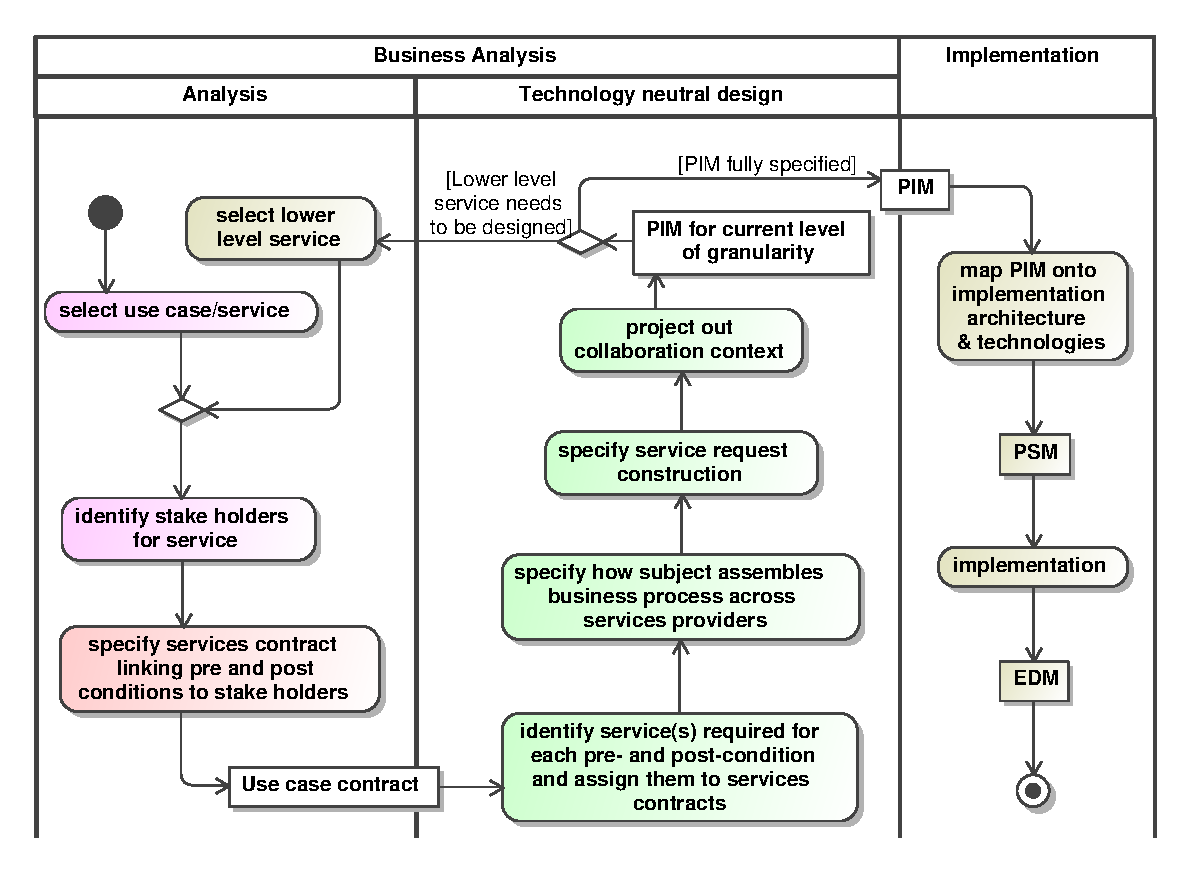
\epsfig{file=methodology.eps}
	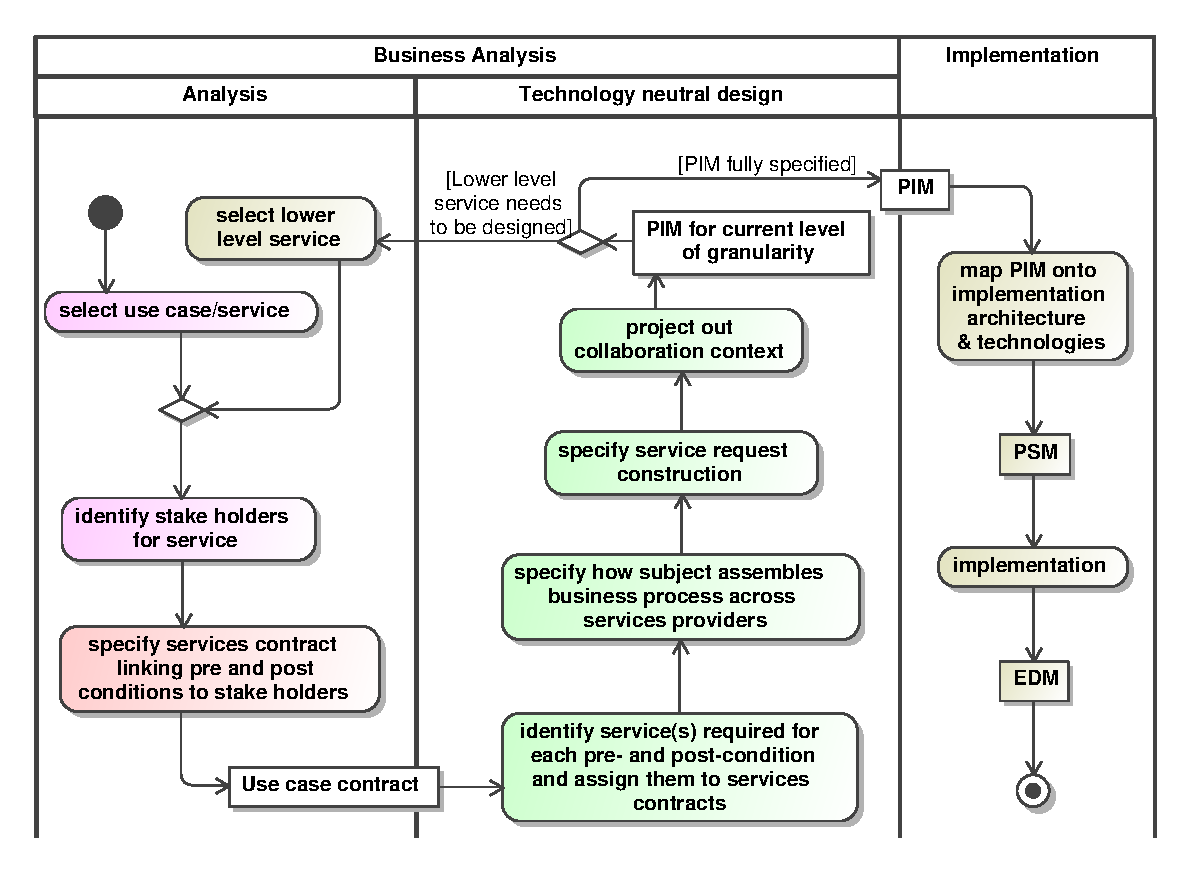
\epsfig{file=methodology.eps, height=3in, width=3.4in}
	\caption{The URDAD process. \label{fig:methodology}}
\end{figure}

The first step in the design phase is to identify the functional requirements for the service, i.e.\ the functions or services required to address the pre- and post-conditions for the service. This introduces the services contracts for the lower level services from which the core service is to be established. For leaf services which are not assembled from lower level services the required logic is fully specified by atomic pre- and post-conditions.

Next one assembles the business process in a UML activity diagram for the higher level service which shows how the process is assembled form the lower level services identified in the previous step. Finally the collaboration context is projected out. The collaboration context shows the services provider contracts with the required services and the required message paths between the service providers.

If any of the lower level services are to be realized within the system, organization or department, then the process is repeated for that lower level service. If the service is to be sourced externally from other systems, departments or external service providers, then one stops after having specified the services contract for that service.

%=============================

\subsection{Structure of an URDAD PIM}

An URDAD PIM encourages parsimony by using a minimal subset of UML. Not only is each model element required, by virtue of the parsimony, but each model element also has a precise semantics. An URDAD PIM has the following elements:
\begin{itemize}
  \item Each required service is specified in a services contract (UML interface) which indicates the inputs and outputs for the service, the pre-and post conditions and the quality requirements specified for the service. The highest level services are the services offered to users.
  \item Each pre and post-condition is the end-point of a {\em requires} dependency leading from the stakeholder(s) who require it. The {\em requires} dependency is defined in the URDAD profile. Stakeholders are to be represented by UML interfaces.
  \item The functionality used to realize each pre- and and post-condition is specified via a {\em requires} dependency pointing to the use case representing the functional requirement.
  \item For each use case, there is a realization relationship from a service in a services contract to the use case.
  \item Concrete service providers are represented by classes which realize/implement services contracts. (Business) processes in the form of activity or sequence diagrams are required to be attached to the services of concrete service providers. These concrete service providers define technology-neutral processes realizing the services in the services contracts.
  \item Services either provide the required output or signal that they will not realize the requested service by throwing an exception. Each exception must be linked to a pre-condition for the service via a usage relationship from the pre-condition to the exception class.
  \item The data structures for all inputs and outputs must be specified.
  \item User roles are represented by interfaces representing user contracts that accumulate the user's obligations around the services used by that user role. The interaction (sequence of messages exchanged) in the context of a user making use of a service specified in a services  contract are specified using a UML sequence diagram.
  \item The effect of atomic/leaf services (services which are not assembled from lower level services) on the environment is fully specified using pre- and post-conditions.
\end{itemize}
